\subsection{Linux versioning scheme and development process}

\begin{frame}
  \frametitle{Linux versioning scheme}
  \begin{itemize}
  \item Until 2003, there was a new ``stabilized'' release branch of Linux every
        2 or 3 years (2.0, 2.2, 2.4). Development branches took 2-3
        years to be merged (too slow!).
  \item Since 2003, there is a new official release of Linux about every
	10 weeks:
  \begin{itemize}
	\item Versions \code{2.6} (Dec. 2003) to \code{2.6.39} (May 2011)
	\item Versions \code{3.0} (Jul. 2011) to \code{3.19} (Feb. 2015)
	\item Versions \code{4.0} (Apr. 2015) to \code{4.20} (Dec. 2018)
	\item Versions \code{5.0} (Mar. 2019) to \code{5.19} (July 2022)
	\item Version \code{6.0} was released in Oct. 2022.
  \end{itemize}
  \item Features are added to the kernel in a progressive way. Since
        2003, kernel developers have managed to do so without having
        to introduce a massively incompatible development branch.
  \item For each release, there are bugfix and security updates called
    stable releases: 6.0.1, 6.0.2, etc.
  \end{itemize}
\end{frame}

\begin{frame}
  \frametitle{Linux development model}
  Using merge and bug fixing windows
  \begin{center}
    \includegraphics[width=\textwidth]{slides/sysdev-linux-intro-versioning/development-process.pdf}
  \end{center}
\end{frame}

\begin{frame}[fragile]
  \frametitle{Need for long term support (1)}
  \begin{itemize}
  \item Issue: bug and security fixes only released for most recent
    kernel versions.
  \item Solution: the last release of each year is made an LTS {\em (Long Term
     Support)} release, and is supposed to be supported (and receive bug
    and security fixes) for up to 6 years.
  \begin{columns}
  \column{0.6\textwidth}
  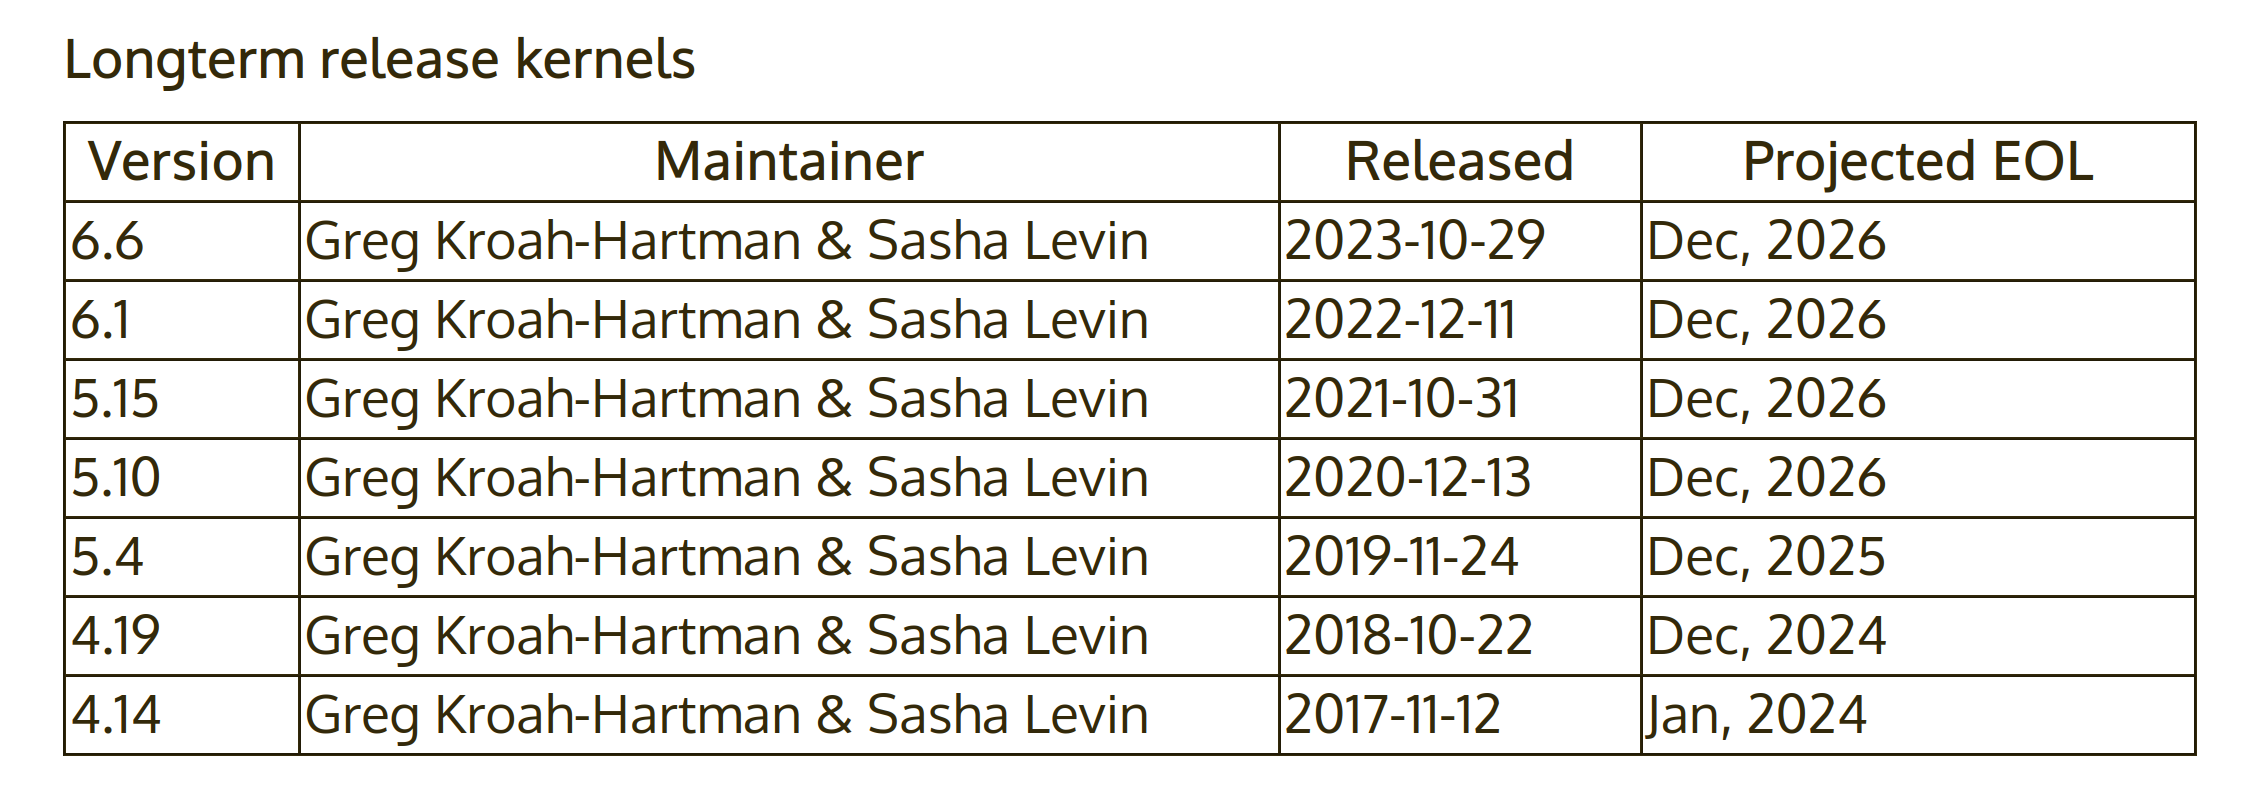
\includegraphics[width=\textwidth]{common/long-term-support-kernels.png}\\
  \column{0.4\textwidth}
  \scriptsize
   Captured on \url{https://kernel.org} in Apr. 2023, following the
   \href{https://www.kernel.org/category/releases.html}{\em Releases} link.
  \end{columns}
  \item Example at Google: starting from {\em Android O (2017)}, all new Android devices will
    have to run such an LTS kernel.
  \end{itemize}
\end{frame}

\begin{frame}[fragile]
  \frametitle{Need for long term support (2)}
  \begin{itemize}
  \item You could also get long term support from a commercial embedded
    Linux provider.
    \begin{itemize}
	\item Wind River Linux can be supported for up to 15 years.
	\item Ubuntu Core can be supported for up to 10 years.
    \end{itemize}
  \item {\em "If you are not using a supported distribution kernel, or a stable / longterm
    kernel, you have an insecure kernel"} - Greg KH, 2019\\
    Some vulnerabilities are fixed in stable without ever getting a CVE.
  \item The {\em Civil Infrastructure Platform} project is an industry /
    Linux Foundation effort to support much longer (at least 10 years)
    selected LTS versions (currently 4.4, 4.19, 5.10) on selected architectures.
    See \url{https://wiki.linuxfoundation.org/civilinfrastructureplatform/cipkernelmaintenance}.
  \end{itemize}
\end{frame}
